%-----------------------------------------------------------------------------------------------%
%
% Maret 2019
% Template Latex untuk Tugas Akhir Program Studi Sistem informasi ini
% dikembangkan oleh Inggih Permana (inggihjava@gmail.com)
%
% Template ini dikembangkan dari template yang dibuat oleh Andreas Febrian (Fasilkom UI 2003).
%
% Orang yang cerdas adalah orang yang paling banyak mengingat kematian.
%
%-----------------------------------------------------------------------------------------------%

%-----------------------------------------------------------------------------------------------%
% Dilarang mengedit file ini, karena dapat merubah format penulisan
%-----------------------------------------------------------------------------------------------%

\documentclass[12pt, a4paper, onecolumn, oneside, final]{report}
\usepackage{kontrol/uinsuskatugasakhir}
%-----------------------------------------------------------------------------------------------%
%
% Maret 2019
% Template Latex untuk Tugas Akhir Program Studi Sistem informasi ini
% dikembangkan oleh Inggih Permana (inggihjava@gmail.com)
%
% Template ini dikembangkan dari template yang dibuat oleh Andreas Febrian (Fasilkom UI 2003).
%
% Orang yang cerdas adalah orang yang paling banyak mengingat kematian.
%
%-----------------------------------------------------------------------------------------------%

%-----------------------------------------------------------------------------------------------%
% Dilarang mengedit file ini, karena dapat merubah format penulisan
%-----------------------------------------------------------------------------------------------%

\var{\fakultas}{Fakultas Sains dan Teknologi}
\var{\fakultasInggris}{Faculty of Science and Technology}

\var{\programStudi}{Sistem Informasi}
\var{\programStudiInggris}{Information System}

\var{\gelar}{Sarjana Komputer}

\var{\universitas}{Universitas Islam Negeri Sultan Syarif Kasim Riau}
\var{\universitasInggris}{\emph{State Islamic University of Sultan Syarif Kasim Riau}}

\var{\kota}{Pekanbaru}

\var{\alamatUniversitas}{Jl. Soebrantas, No. 155, Pekanbaru}
\var{\alamatUniversitasInggris}{\emph{Soebrantas Street, No. 155, Pekanbaru}}

\var{\kaprodi}{Idria Maita, S.Kom., M.Sc.}
\var{\kaprodinip}{197905132007102005}

\var{\dekan}{Dr. Drs. Ahmad Darmawi, M.Ag.}
\var{\dekannip}{196606041992031004}

\var{\rektor}{Prof. Dr. H. Akhmad Mujahidin, S.Ag., M.Ag.}
\var{\rektorSatu}{Dr. Drs. H. Suryan A. Jamrah, MA.}
\var{\rektorDua}{Dr. H. Kusnadi, M.Pd.}
\var{\rektorTiga}{Drs. H. Promadi, MA., Ph.D.}

%-----------------------------------------------------------------------------%
% Judul BAB
%-----------------------------------------------------------------------------%
%

\Var{\lembarPersetujuan}{LEMBAR PERSETUJUAN}
\Var{\lembarPengesahan}{LEMBAR PENGESAHAN}
\Var{\kataPengantar}{Kata Pengantar}
\Var{\babSatu}{Pendahuluan}
\Var{\babDua}{Landasan Teori}
\Var{\babTiga}{Metodologi Penelitian}
\Var{\babEmpat}{Analisa dan Perancangan}
\Var{\babLima}{Implementasi dan Pengujian}
\Var{\babEnam}{Penutup}
%-----------------------------------------------------------------------------------------------%
%
% Maret 2019
% Template Latex untuk Tugas Akhir Program Studi Sistem informasi ini
% dikembangkan oleh Inggih Permana (inggihjava@gmail.com)
%
% Template ini dikembangkan dari template yang dibuat oleh Andreas Febrian (Fasilkom UI 2003).
%
% Orang yang cerdas adalah orang yang paling banyak mengingat kematian.
%
%-----------------------------------------------------------------------------------------------%
 
\var{\judul}{AUDIT KEAMANAN INFORMASI SISTEM INFORMASI KASTAMER PADA UNIT \textit{PAYMENT COLLECTION} MENGGUNAKAN STANDAR ISO 27001}
\var{\judulInggris}{\textit{CARA MEMBUAT TUGAS AKHIR PROGRAM STUDI SISTEM INFORMASI MENGGUNAKAN latex}}
\var{\penulis}{VELLA HERMAN}
\var{\email}{fathirpermana@uin-suska.ac.id}
\var{\nohp}{0852XXXXXXXX}
\var{\nim}{11453201711}
\var{\tahun}{2020}
\var{\pengujipertama}{Tengku Khairil Ahsyar, M.Kom.}
\var{\pengujikedua}{Mustakim, ST., M.Kom.}

\var{\pembimbingpertama}{Inggih Permana, ST., M.Kom.}
\var{\pembimbingpertamanip}{198812102015031006}
% Isi prefik pembimbing pertama dengan "NIP" atau "NIK", tanpa tanda kutip
% Silahkan tanya pembimbing anda
\var{\prefiknomorinduksatu}{NIP}

% Jika tidak ada pembimbing 2 silahkan isi dengan -- saja
\var{\pembimbingkedua}{M. Afdal, ST., M.Kom.}
\var{\pembimbingkeduanip}{151XXXXXX}
% Isi prefik pembimbing kedua dengan "NIP" atau "NIK", tanpa tanda kutip
% Silahkan tanya pembimbing anda
\var{\prefiknomorindukdua}{NIK}

\var{\ketuaSidang}{Nurmaini Dalimunthe, M.Kes.}

\var{\tanggalPersetujuan}{27 Desember 2016}

\var{\tanggalSidang}{20 Desember 2016}
\var{\tanggalSidangInggris}{December 20$^{th}$ 2016}

% Tipe diisi dengan "TUGAS AKHIR" atau "PROPOSAL TUGAS AKHIR", tanpa tanda kutip
\var{\tipeta}{PROPOSAL TUGAS AKHIR}

% Jumlah pembimbing, isi dengan kata "SATU" atau "DUA", tanpa tanda kutip
\var{\jumlahpembimbing}{SATU}

% Isi bidang TA dengan "SATU" atau "DUA", tanpa tanda kutip
% SATU untuk TA bidang RSI (6 BAB)
% DUA untuk TA bidang MSI, BSI, DAMING dan yang sejenis (5 BAB)
\var{\bidangta}{DUA}
%-----------------------------------------------------------------------------------------------%
%
% Maret 2019
% Template Latex untuk Tugas Akhir Program Studi Sistem informasi ini
% dikembangkan oleh Inggih Permana (inggihjava@gmail.com)
%
% Template ini dikembangkan dari template yang dibuat oleh Andreas Febrian (Fasilkom UI 2003).
%
% Orang yang cerdas adalah orang yang paling banyak mengingat kematian.
%
%-----------------------------------------------------------------------------------------------%

\hyphenation{
    % alphabhet A
    a-na-li-sa a-tur 
    a-pli-ka-si 
    % alphabhet B
    ba-ngun-an 
    be-be-ra-pa 
    ber-ge-rak
    ber-ke-lan-jut-an 
    ber-pe-nga-ruh 
    % alphabhet C
    ca-ri
    % alphabhet D
    di-sim-pan di-pim-pin de-ngan da-e-rah di-ba-ngun da-pat di-nya-ta-kan 
    di-sim-bol-kan di-pi-lih di-li-hat de-fi-ni-si
    % alphabhet E
    e-ner-gi eks-klu-sif
    % alphabhet F
    fa-si-li-tas
    % alphabhet G
    ga-bung-an ge-rak
    % alphabhet H
    ha-lang-an
    % alphabhet I
    % alphabhet J
    % alphabhet K
    ke-hi-lang-an
    ku-ning 
    kua-li-tas ka-me-ra ke-mung-kin-an ke-se-pa-ham-an
    ka-la-ngan
    % alphabhet L
    ling-kung-an
    % alphabhet M
    me-neng-ah
    meng-a-tas-i me-mung-kin-kan me-nge-na-i me-ngi-rim-kan 
    meng-u-bah meng-a-dap-ta-si me-nya-ta-kan mo-di-fi-ka-si
    meng-a-tur
    me-min-jam-kan
    % alphabhet N
    nya-ta non-eks-klu-sif
    % alphabhet O
    % alphabhet P
	pe-nye-rap-an 
	pe-ngon-trol
    pe-mo-del-an
    pe-ran  pe-ran-an-nya
    pem-ba-ngun-an pre-si-den pe-me-rin-tah prio-ri-tas peng-am-bil-an 
    peng-ga-bung-an pe-nga-was-an pe-ngem-bang-an 
    pe-nga-ruh pa-ra-lel-is-me per-hi-tung-an per-ma-sa-lah-an 
    pen-ca-ri-an peng-struk-tur-an
    % alphabhet Q
    % alphabhet R
    ran-cang-an
    % alphabhet S
    si-mu-la-si sa-ngat
    % alphabhet T
    te-ngah
    ter-da-pat
    % alphabhet U
    % alphabhet V
    % alphabhet W
    % alphabhet X
    % alphabhet Y
    % alphabhet Z
    % special
} 
%-----------------------------------------------------------------------------------------------%
%
% Maret 2019
% Template Latex untuk Tugas Akhir Program Studi Sistem informasi ini
% dikembangkan oleh Inggih Permana (inggihjava@gmail.com)
%
% Template ini dikembangkan dari template yang dibuat oleh Andreas Febrian (Fasilkom UI 2003).
%
% Orang yang cerdas adalah orang yang paling banyak mengingat kematian.
%
%-----------------------------------------------------------------------------------------------%

\var{\license}{\f{Creative Common License 1.0 Generic}}
\var{\bslash}{$\setminus$}


\begin{document}
\renewcommand{\BBAB}{dan}
\renewcommand{\BBAA}{dan}
\renewcommand{\BOthers}[1]{dkk.\hbox{}}
\renewcommand{\BOthersPeriod}[1]{dkk.\hbox{}}
\renewcommand{\BIn}{Dalam}
\renewcommand{\BPG}{hal.\hbox{}}
\renewcommand{\BPGS}{hal.\hbox{}} 

%-----------------------------------------------------------------------------------------------%%
% Maret 2019
% Template Latex untuk Tugas Akhir Program Studi Sistem informasi ini
% dikembangkan oleh Inggih Permana (inggihjava@gmail.com)
%
% Template ini dikembangkan dari template yang dibuat oleh Andreas Febrian (Fasilkom UI 2003).
%
% Orang yang cerdas adalah orang yang paling banyak mengingat kematian.
%
%-----------------------------------------------------------------------------------------------%

%-----------------------------------------------------------------------------------------------%
% Dilarang mengedit file ini, karena dapat merubah format penulisan
%-----------------------------------------------------------------------------------------------%

\begin{titlepage}
    \begin{center}
    	\fontsize{14pt}{16.8pt}\selectfont\MakeUppercase{\bo{\judul}}\\
        \vspace{1.5cm}
        \fontsize{16pt}{19.2pt}\selectfont\MakeUppercase{\bo{\tipeta}}\\
        \vspace{1.5cm}
        \fontsize{11pt}{13.2pt}\selectfont Diajukan Sebagai Salah Satu Syarat\\
        untuk Memperoleh Gelar \gelar \space \normalfont{pada}\\
        Program Studi \programStudi\\
        \vspace{1.5cm}

        \fontsize{13.5pt}{16.2pt}\selectfont Oleh:\\
        % \vspace{1.0cm}
        \MakeUppercase{\bo{\underline{\penulis}}}\\
        \MakeUppercase{\bo{\nim}}\\
       

       \vfill
       \vspace{1.5cm}
       
\includegraphics[width=5.2cm, height=5.2cm]{kontrol/gambar/logouin.png}
       \vspace{1.5cm}
       \vfill
 
         \fontsize{13.5pt}{16.2pt}\selectfont\MakeUppercase{\bo{\fakultas}}\\
         \MakeUppercase{\bo{\universitas}}\\
         \MakeUppercase{\bo{\kota}}\\
         \bo{\tahun}\\
    \end{center}
\end{titlepage}


\pagenumbering{roman}

\setcounter{page}{2}
\ifthenelse{\equal{\tipeta}{TUGAS AKHIR}}{
  \ifthenelse{\equal{\jumlahpembimbing}{SATU}}{
    \addChapter{\lembarPersetujuan}
    %-----------------------------------------------------------------------------------------------%
%
% Maret 2019
% Template Latex untuk Tugas Akhir Program Studi Sistem informasi ini
% dikembangkan oleh Inggih Permana (inggihjava@gmail.com)
%
% Template ini dikembangkan dari template yang dibuat oleh Andreas Febrian (Fasilkom UI 2003).
%
% Orang yang cerdas adalah orang yang paling banyak mengingat kematian.
%
%-----------------------------------------------------------------------------------------------%

%-----------------------------------------------------------------------------------------------%
% Dilarang mengedit file ini, karena dapat merubah format penulisan
%-----------------------------------------------------------------------------------------------%

\chapter*{\lembarPersetujuan}
\begin{center}
\fontsize{14pt}{16.8pt}\selectfont\MakeUppercase{\bo{\judul}}\\

      \vspace{1.5cm}
      \fontsize{14pt}{16.8pt}\selectfont\MakeUppercase{\bo {Tugas Akhir}}\\
      \vspace{1.5cm}

        Oleh:\\
        \vspace{1.0cm}
        \MakeUppercase{\bo{\underline{\penulis}}}\\
        \MakeUppercase{\bo{\nim}}\\
      \vspace{1.5cm}

      \fontsize{12pt}{14.4pt}\selectfont Telah diperiksa dan disetujui sebagai laporan tugas akhir\\
      \fontsize{12pt}{14.4pt}\selectfont di \kota, pada tanggal \tanggalPersetujuan\\
      \vspace{1.5cm}
  
    \begin{tabular}{lll}
      \bo{Ketua Program Studi} & \hspace{2cm} & \bo{Pembimbing} \\
      \vspace{0.5cm} & \vspace{0.5cm} & \vspace{0.5cm}\\
      \bo{\underline{\kaprodi}}& & \bo{\underline{\pembimbingpertama}} \\
      \bo {NIP. \kaprodinip} & & \bo {\prefiknomorinduksatu. \pembimbingpertamanip}    
    \end{tabular}
    \end{center}

    \addChapter{\lembarPengesahan}
    %-----------------------------------------------------------------------------------------------%
%
% Maret 2019
% Template Latex untuk Tugas Akhir Program Studi Sistem informasi ini
% dikembangkan oleh Inggih Permana (inggihjava@gmail.com)
%
% Template ini dikembangkan dari template yang dibuat oleh Andreas Febrian (Fasilkom UI 2003).
%
% Orang yang cerdas adalah orang yang paling banyak mengingat kematian.
%
%-----------------------------------------------------------------------------------------------%

%-----------------------------------------------------------------------------------------------%
% Dilarang mengedit file ini, karena dapat merubah format penulisan
%-----------------------------------------------------------------------------------------------%

\chapter*{\lembarPengesahan}
\begin{center}
    \fontsize{14pt}{16.8pt}\selectfont
    \MakeUppercase{\bo{\judul}}\\

      \vfill
      \MakeUppercase{\bo{Tugas Akhir}}\\
      \vfill

        Oleh:\\
        \vfill
        \MakeUppercase{\bo{\underline{\penulis}}}\\
        \MakeUppercase{\bo{\nim}}\\
      \vfill

      \fontsize{12pt}{14.4pt}\selectfont\normalfont Telah dipertahankan di depan sidang dewan penguji\\
      sebagai salah satu syarat untuk memperoleh gelar \gelar\\
      \fakultas \space \universitas\\
      di \kota, pada tanggal \tanggalSidang\\
      \vfill
  
  \begin{tabular}{l}
    \begin{tabular}{lll}
      & & \kota, \tanggalSidang \\
       & & Mengesahkan,\\
       & &  \\
      \bo{Dekan} & \hspace{2cm} & \bo{Ketua Program Studi} \\
      \vspace{0.5cm} & \vspace{0.5cm} & \vspace{0.5cm}\\
      \bo{\underline{\dekan}}& &
      \bo{\underline{\kaprodi}} \\
      \bo{NIP. \dekannip} & & \bo{NIP. \kaprodinip}    
    \end{tabular} \\ \\
    \normalfont{
  \begin{tabular}{llrr}
    \multicolumn{4}{l}{\bo{DEWAN PENGUJI:}}\\
    \bo{Ketua} & \bo{:} \bo{\ketuaSidang} & \underline{\space \space \space\space \space \space\space \space \space\space \space \space\space \space \space\space \space \space\space \space \space} & \\
    & & & \\
    \bo{Sekretaris} & \bo{:} \bo{\pembimbingpertama} & & \underline{\space \space \space\space \space \space\space \space \space\space \space \space\space \space \space\space \space \space\space \space \space}\\
    & & & \\
    \bo{Anggota 1} & \bo{:} \bo{\pengujipertama} & \underline{\space \space \space\space \space \space\space \space \space\space \space \space\space \space \space\space \space \space\space \space \space} & \\
    & & & \\
    \bo{Anggota 2} & \bo{:} \bo{\pengujikedua} & & \underline{\space \space \space\space \space \space\space \space \space\space \space \space\space \space \space\space \space \space\space \space \space}\\
   \end{tabular}
   }
   \end{tabular}

  \end{center}
  }
  {
    \addChapter{\lembarPersetujuan}
    %-----------------------------------------------------------------------------------------------%
%
% Maret 2019
% Template Latex untuk Tugas Akhir Program Studi Sistem informasi ini
% dikembangkan oleh Inggih Permana (inggihjava@gmail.com)
%
% Template ini dikembangkan dari template yang dibuat oleh Andreas Febrian (Fasilkom UI 2003).
%
% Orang yang cerdas adalah orang yang paling banyak mengingat kematian.
%
%-----------------------------------------------------------------------------------------------%

%-----------------------------------------------------------------------------------------------%
% Dilarang mengedit file ini, karena dapat merubah format penulisan
%-----------------------------------------------------------------------------------------------%

\chapter*{\lembarPersetujuan}
\begin{center}
\fontsize{14pt}{16.8pt}\selectfont\MakeUppercase{\bo{\judul}}\\

      \vspace{1.5cm}
      \fontsize{14pt}{16.8pt}\selectfont\MakeUppercase{\bo {Tugas Akhir}}\\
      \vspace{1.5cm}

        Oleh:\\
        \vspace{1.0cm}
        \MakeUppercase{\bo{\underline{\penulis}}}\\
        \MakeUppercase{\bo{\nim}}\\
      \vspace{1.5cm}

      \fontsize{12pt}{14.4pt}\selectfont Telah diperiksa dan disetujui sebagai laporan tugas akhir\\
      \fontsize{12pt}{14.4pt}\selectfont di \kota, pada tanggal \tanggalPersetujuan\\
      \vspace{1.5cm}
  
    \begin{tabular}{lll}
      \bo{Pembimbing I} & \hspace{2cm} & \bo{Pembimbing II} \\
      \vspace{0.5cm} & \vspace{0.5cm} & \vspace{0.5cm}\\
      \bo{\underline{\pembimbingpertama}}& & \bo{\underline{\pembimbingkedua}} \\
      \bo {\prefiknomorinduksatu . \pembimbingpertamanip} & & \bo {\prefiknomorindukdua . \pembimbingkeduanip}    
    \end{tabular}

    \vspace{1cm}
    \begin{tabular}{l}
      \bo{Ketua Program Studi}\\
      \vspace{1.5cm}\\
      \bo{\underline{\kaprodi}}\\
      \bo {NIP. \kaprodinip}    
    \end{tabular}

    \end{center}

    \addChapter{\lembarPengesahan}
    %-----------------------------------------------------------------------------------------------%
%
% Maret 2019
% Template Latex untuk Tugas Akhir Program Studi Sistem informasi ini
% dikembangkan oleh Inggih Permana (inggihjava@gmail.com)
%
% Template ini dikembangkan dari template yang dibuat oleh Andreas Febrian (Fasilkom UI 2003).
%
% Orang yang cerdas adalah orang yang paling banyak mengingat kematian.
%
%-----------------------------------------------------------------------------------------------%

%-----------------------------------------------------------------------------------------------%
% Dilarang mengedit file ini, karena dapat merubah format penulisan
%-----------------------------------------------------------------------------------------------%

\chapter*{\lembarPengesahan}
\begin{center}
    \fontsize{14pt}{16.8pt}\selectfont
    \MakeUppercase{\bo{\judul}}\\

      \vfill
      \MakeUppercase{\bo{Tugas Akhir}}\\
      \vfill

        Oleh:\\
        \vfill
        \MakeUppercase{\bo{\underline{\penulis}}}\\
        \MakeUppercase{\bo{\nim}}\\
      \vfill

      \fontsize{12pt}{14.4pt}\selectfont\normalfont Telah dipertahankan di depan sidang dewan penguji\\
      sebagai salah satu syarat untuk memperoleh gelar \gelar\\
      \fakultas \space \universitas\\
      di \kota, pada tanggal \tanggalSidang\\
      \vfill
  
  \begin{tabular}{l}
    \begin{tabular}{lll}
      & & \kota, \tanggalSidang \\
       & & Mengesahkan,\\
       & &  \\
      \bo{Dekan} & \hspace{2cm} & \bo{Ketua Program Studi} \\
      \vspace{0.5cm} & \vspace{0.5cm} & \vspace{0.5cm}\\
      \bo{\underline{\dekan}}& &
      \bo{\underline{\kaprodi}} \\
      \bo{NIP. \dekannip} & & \bo{NIP. \kaprodinip}    
    \end{tabular} \\ \\
    \normalfont{
  \begin{tabular}{llrr}
    \multicolumn{4}{l}{\bo{DEWAN PENGUJI:}}\\
    \bo{Ketua} & \bo{:} \bo{\ketuaSidang} & \underline{\space \space \space\space \space \space\space \space \space\space \space \space\space \space \space\space \space \space\space \space \space} & \\
    & & & \\
    \bo{Sekretaris} & \bo{:} \bo{\pembimbingpertama} & & \underline{\space \space \space\space \space \space\space \space \space\space \space \space\space \space \space\space \space \space\space \space \space}\\
    & & & \\
    \bo{Anggota 1} & \bo{:} \bo{\pembimbingkedua} & \underline{\space \space \space\space \space \space\space \space \space\space \space \space\space \space \space\space \space \space\space \space \space} & \\
    & & & \\
    \bo{Anggota 2} & \bo{:} \bo{\pengujipertama} & & \underline{\space \space \space\space \space \space\space \space \space\space \space \space\space \space \space\space \space \space\space \space \space}\\
    & & & \\ 
    \bo{Anggota 3} & \bo{:} \bo{\pengujikedua} & \underline{\space \space \space\space \space \space\space \space \space\space \space \space\space \space \space\space \space \space\space \space \space} & 
   \end{tabular}
   }
   \end{tabular}

  \end{center}
  }

\addChapter{LEMBAR HAK ATAS KEKAYAAN INTELEKTUAL}
%-----------------------------------------------------------------------------------------------%
%
% Maret 2019
% Template Latex untuk Tugas Akhir Program Studi Sistem informasi ini
% dikembangkan oleh Inggih Permana (inggihjava@gmail.com)
%
% Template ini dikembangkan dari template yang dibuat oleh Andreas Febrian (Fasilkom UI 2003).
%
% Orang yang cerdas adalah orang yang paling banyak mengingat kematian.
%
%-----------------------------------------------------------------------------------------------%

%-----------------------------------------------------------------------------------------------%
% Dilarang mengedit file ini, karena dapat merubah format penulisan
%-----------------------------------------------------------------------------------------------%

\chapter*{LEMBAR HAK ATAS KEKAYAAN INTELEKTUAL}

Tugas Akhir yang tidak diterbitkan ini terdaftar dan tersedia di Perpustakaan Universitas Islam Negeri Sultan Syarif Kasim Riau adalah terbuka untuk umum, dengan ketentuan bahwa hak cipta ada pada penulis. Referensi kepustakaan diperkenankan dicatat, tetapi pengutipan atau ringkasan hanya dapat dilakukan atas izin penulis dan harus dilakukan mengikuti kaedah dan kebiasaan ilmiah serta menyebutkan sumbernya.

Penggandaan atau penerbitan sebagian atau seluruh Tugas Akhir ini harus memperoleh izin tertulis dari Dekan \@fakultas \@universitas. Perpustakaan dapat meminjamkan Tugas Akhir ini untuk anggotanya dengan mengisi nama, tanda peminjaman dan tanggal pinjam pada \emph{form} peminjaman.

\addChapter{LEMBAR PERNYATAAN}
%-----------------------------------------------------------------------------------------------%
%
% Maret 2019
% Template Latex untuk Tugas Akhir Program Studi Sistem informasi ini
% dikembangkan oleh Inggih Permana (inggihjava@gmail.com)
%
% Template ini dikembangkan dari template yang dibuat oleh Andreas Febrian (Fasilkom UI 2003).
%
% Orang yang cerdas adalah orang yang paling banyak mengingat kematian.
%
%-----------------------------------------------------------------------------------------------%

%-----------------------------------------------------------------------------------------------%
% Dilarang mengedit file ini, karena dapat merubah format penulisan
%-----------------------------------------------------------------------------------------------%

\chapter*{LEMBAR PERNYATAAN}

Dengan ini saya menyatakan bahwa dalam Tugas Akhir ini tidak terdapat karya yang pernah diajukan untuk memperoleh gelar kesarjanaan di suatu Perguruan Tinggi, dan sepanjang pengetahuan saya juga tidak terdapat karya atau pendapat yang pernah ditulis atau diterbitkan oleh orang lain kecuali yang secara tertulis diacu dalam naskah ini dan disebutkan di dalam daftar pustaka.\\
\vspace{1cm}\\
\begin{tabular}{cc}
      \hspace{8cm} & \ \kota, \tanggalSidang\\
      & \ Yang membuat pernyataan,\\
      \vspace{0.5cm} & \vspace{0.5cm}\\
      & \textbf{\underline{\penulis}} \\
      & \textbf {NIM. \nim}
    \end{tabular}


\addChapter{LEMBAR PERSEMBAHAN}
%-----------------------------------------------------------------------------------------------%
%
% Maret 2019
% Template Latex untuk Tugas Akhir Program Studi Sistem informasi ini
% dikembangkan oleh Inggih Permana (inggihjava@gmail.com)
%
% Template ini dikembangkan dari template yang dibuat oleh Andreas Febrian (Fasilkom UI 2003).
%
% Orang yang cerdas adalah orang yang paling banyak mengingat kematian.
%
%-----------------------------------------------------------------------------------------------%

\chapter*{LEMBAR PERSEMBAHAN}
Tugas akhir ini aku persembahkan untuk ibuku, ayahku, istriku, anak-anakku dan adik-adikku tercinta...

\addChapter{\kataPengantar}
%-----------------------------------------------------------------------------------------------%
%
% Maret 2019
% Template Latex untuk Tugas Akhir Program Studi Sistem informasi ini
% dikembangkan oleh Inggih Permana (inggihjava@gmail.com)
%
% Template ini dikembangkan dari template yang dibuat oleh Andreas Febrian (Fasilkom UI 2003).
%
% Orang yang cerdas adalah orang yang paling banyak mengingat kematian.
%
%-----------------------------------------------------------------------------------------------%

%-----------------------------------------------------------------------------%
\chapter*{\kataPengantar}
%-----------------------------------------------------------------------------%
Tulis kata pengantar anda di bagian ini. Ucapan terima kasih wajib diucapkan pada:
\begin{enumerate}
	\item Bapak \rektor, sebagai Rektor \universitas. 
	\item Bapak \dekan, sebagai Dekan \fakultas. 
	\item Ibu \kaprodi, sebagai Ketua Program Studi \programStudi.
	\item Bapak \pembimbingpertama, sebagai dosen pembimbing tugas akhir ini.
	\item Selanjutnya terserah anda...
\end{enumerate}


Tambah paragraf penutup disini. Tambah paragraf penutup disini. Tambah paragraf penutup disini.
Tambah paragraf penutup disini. Tambah paragraf penutup disini. Tambah paragraf penutup disini.

\vspace*{0.1cm}

\begin{flushright}
\kota, \tanggalPersetujuan\\
Penulis,\\
\vspace{2cm}
\textbf{\underline{\penulis}\\
NIM. \nim}

\end{flushright}

 
\addChapter{ABSTRAK}
%-----------------------------------------------------------------------------------------------%
%
% Maret 2019
% Template Latex untuk Tugas Akhir Program Studi Sistem informasi ini
% dikembangkan oleh Inggih Permana (inggihjava@gmail.com)
%
% Template ini dikembangkan dari template yang dibuat oleh Andreas Febrian (Fasilkom UI 2003).
%
% Orang yang cerdas adalah orang yang paling banyak mengingat kematian.
%
%-----------------------------------------------------------------------------------------------%

\chapter*{\MakeUppercase{\judul}}

\fontsize{14}{16.8}
\begin{center}
	\vspace{0.3cm}
	\MakeUppercase{\textbf{\penulis}}\\
	\MakeUppercase{\textbf{NIM: \nim}}\\
	\fontsize{12}{14.4}
	\vspace{0.7cm}

	Tanggal Sidang: \tanggalSidang\\
	Periode Wisuda:\ \ \ \ \ \ \ \ \ \ \ \ \ \ \ \ \ \ \ \ \ \ \ \ \ \ \ \ \ \ \ \ \ \ \ \ \ \ 

	\vspace{0.7cm}
	Program Studi \programStudi\\
	\fakultas\\
	\universitas\\
	\alamatUniversitas\\

	\vspace{0.7cm}
\end{center}

\fontsize{12}{14.4}
\begin{center}\MakeUppercase{\textbf{Abstrak}}\end{center}

\noindent
\fontsize{10pt}{12pt}\selectfont
Salah satu hewan yang sering dijadikan kurban pada saat hari raya Idul Adha adalah sapi. Ada banyak kriteria yang harus diperhatikan dalam menentukan kelayakan seekor sapi untuk dijadikan kurban. Kriteria-kriteria tersebut sering diabaikan oleh masyarakat. Hal ini dikarenakan ketidaktahuan masyarakat tentang kriteria-kriteria tersebut. Disamping itu, jumlah pakar yang bisa menilai kelayakan hewan kurban dan mensosialisasikan hal tersebut ke masyarakat sangat terbatas. DST... (Maksimal 200 kata)\\
\noindent{\textbf{Kata Kunci:} \textit{forward chaining}, sapi, DST (Maksimal 5)} \\

\addChapter{\emph{ABSTRACT}}
%-----------------------------------------------------------------------------------------------%
%
% Maret 2019
% Template Latex untuk Tugas Akhir Program Studi Sistem informasi ini
% dikembangkan oleh Inggih Permana (inggihjava@gmail.com)
%
% Template ini dikembangkan dari template yang dibuat oleh Andreas Febrian (Fasilkom UI 2003).
%
% Orang yang cerdas adalah orang yang paling banyak mengingat kematian.
%
%-----------------------------------------------------------------------------------------------%

\chapter*{\MakeUppercase{\textit{\judulInggris}}}

\fontsize{14}{16.8}
\begin{center}
	\vspace{0.3cm}
	\MakeUppercase{\textbf{\penulis}}\\
	\MakeUppercase{\textbf{NIM: \nim}}\\
	\fontsize{12}{14.4}
	\vspace{0.7cm}

	\textit{Date of Final Exam: \tanggalSidangInggris}\\
	\textit{Graduation Period:}\ \ \ \ \ \ \ \ \ \ \ \ \ \ \ \ \ \ \ \ \ \ \ \ \ \ \ \ \ \ \ \ \ \ \ \ \ \ 

	\vspace{0.7cm}
	\emph{Department of \programStudiInggris}\\
	\textit{\fakultasInggris}\\
	\universitasInggris\\
	\alamatUniversitasInggris\\

	\vspace{0.7cm}
\end{center}

\fontsize{12}{14.4}
\begin{center}\MakeUppercase{\textbf{\emph{Abstract}}}\end{center}

\noindent
\fontsize{10pt}{12pt}\selectfont
\emph{One of the animals that are often used as a sacrifice at the time of the feast of Eid al-Adha is a cow there are many criteria that must be considered in determining the eligibility of a cow to be made a sacrifice of such criteria is often overlooked by the public this is due to the ignorance of people about these criteria. In addition, the number of experts who can assess the feasibility of sacrificial animals and disseminating it to the public is very limited. This research has made the mobile-based expert system for determining the eligibility of cattle a sacrifice so that the community can help to determine the feasibility of a sacrificial cow.}\\
\noindent{\emph{\textbf{Keywords:} forward chaining, cow, DST (Maksimal 5)}} \\
}{}

\fontsize{12pt}{14.4pt}\selectfont

\phantomsection
\tableofcontents
\clearpage
\phantomsection
\listoffigures
\clearpage
\phantomsection
\listoftables
\clearpage

\addChapter{DAFTAR SINGKATAN}
%-----------------------------------------------------------------------------------------------%
%
% Maret 2019
% Template Latex untuk Tugas Akhir Program Studi Sistem informasi ini
% dikembangkan oleh Inggih Permana (inggihjava@gmail.com)
%
% Template ini dikembangkan dari template yang dibuat oleh Andreas Febrian (Fasilkom UI 2003).
%
% Orang yang cerdas adalah orang yang paling banyak mengingat kematian.
%
%-----------------------------------------------------------------------------------------------%

%-----------------------------------------------------------------------------%
\chapter*{DAFTAR SINGKATAN}
%-----------------------------------------------------------------------------%
\begin{tabular}{lll}
AYM &:& Ayam\\
MKN &:& Makan\\
NSI &:& Nasi\\
\end{tabular}
\renewcommand{\headrulewidth}{0.0pt}
  \fancyhf{} 
  \fancyhead[L]{} 
  \fancyhead[C]{} 
  \fancyhead[R]{}
  \fancyfoot[C]{}
  \fancyfoot[R]{\thepage} 
  \renewcommand{\headrulewidth}{0.0pt}  
  \renewcommand{\footrulewidth}{0.0pt} 
\pagestyle{fancy}

\makeatletter
\renewcommand\chapter{\if@openright\cleardoublepage\else\clearpage\fi
                    % \thispagestyle{empty}%
                    \global\@topnum\z@
                    \@afterindentfalse
                    \secdef\@chapter\@schapter}
\makeatother

\fontsize{12pt}{14.4pt}\selectfont

\pagenumbering{arabic}
%-----------------------------------------------------------------------------------------------%
%
% Maret 2019
% Template Latex untuk Tugas Akhir Program Studi Sistem informasi ini
% dikembangkan oleh Inggih Permana (inggihjava@gmail.com)
%
% Template ini dikembangkan dari template yang dibuat oleh Andreas Febrian (Fasilkom UI 2003).
%
% Orang yang cerdas adalah orang yang paling banyak mengingat kematian.
%
%-----------------------------------------------------------------------------------------------%

%-----------------------------------------------------------------------------%
\chapter{\babSatu}
%-----------------------------------------------------------------------------%

%-----------------------------------------------------------------------------%
\section{Latar Belakang}
%-----------------------------------------------------------------------------%
Meningkatnya kesadaran berqurban menjadikan peserta qurban bertambah setiap tahun \cite{mangalagowri2016eeg}. Peserta qurban bukan didominasi lagi oleh kalangan menengah ke atas, namun juga diikuti oleh masyarakat yang memprioritaskan dana yang dimiliki untuk berqurban. Selain itu, perekonomian yang semakin membaik \textit{juga} menjadi \textit{faktor meningkatnya} partisipasi masyarakat dalam berqurban.

Salah satu hewan yang sering dijadikan pilihan qurban adalah sapi. Sapi selalu menjadi langganan qurban di saat hari raya Idul Adha. Hal ini dapat dibuktikan pada setiap Mesjid yang terdapat di sekitar kota Pekanbaru, sapi menjadi mayoritas hewan yang akan disembelih pada hari raya Idul Adha dibandingkan hewan-hewan lainnya seperti kerbau dan kambing. Menurut \citeA{purnamasari2015aspects}, berdasarkan data dari tahun 2011 sampai 2014 menunjukkan bahwa dari 390 Mesjid yang terdapat di Pekanbaru rata-rata mengalami peningkatan penyembelihan sapi.


%-----------------------------------------------------------------------------%
\section{Perumusan Masalah}
%-----------------------------------------------------------------------------%
Perumusan masalah tugas akhir ini adalah bagaimana mengakuisisi kemampuan pakar-pakar yang berhubungan dengan kelayakan sapi qurban ke dalam sebuah basis pengetahuan dan mengimplementasikan basis pengetahuan tersebut ke dalam sistem berbasis mobile.


%-----------------------------------------------------------------------------%
\section{Batasan Masalah}
%-----------------------------------------------------------------------------%
Batasan masalah tugas akhir ini adalah:
\begin{enumerate}
	\item Pakar-pakar pada penelitian ini meliputi pakar peternakan, kesehatan hewan, dan syariah Islam.
	\item Sistem \textit{operasi} \textbf{smartphone} mobile yang digunakan adalah Android Lollipop.
	\item DST...
\end{enumerate}

%-----------------------------------------------------------------------------%
\section{Tujuan}
%-----------------------------------------------------------------------------%
Tujuan tugas akhir ini adalah:
\begin{enumerate}
	\item Tujuan 1.
	\item Tujuan 2.
	\item Tujuan 3.
	\item DST...
\end{enumerate}

%-----------------------------------------------------------------------------%
\section{Manfaat}
%-----------------------------------------------------------------------------%
Manfaat tugas akhir ini adalah:
\begin{enumerate}
	\item Tujuan 1.
	\item Tujuan 2.
	\item DST...
\end{enumerate}

%-----------------------------------------------------------------------------%
\section{Sistematika Penulisan}
%-----------------------------------------------------------------------------%
Sistematika penulisan laporan adalah sebagai berikut:

\textbf{BAB 1. \babSatu}

BAB 1 pada tugas akhir ini berisi tentang: (1) latar belakang masalah; (2) rumusan masalah; (3) batasan masalah; (4) tujuan; (5) manfaat; dan (6) sistematika penulisan.

\textbf{BAB 2. \babDua}

BAB 2 pada tugas akhir ini berisi tentang: DST.


\textbf{BAB 3. \babTiga}

BAB 3 pada tugas akhir ini berisi tentang: DST.


\textbf{BAB 4. \babEmpat}

BAB 4 pada tugas akhir ini berisi tentang: DST.

\textbf{BAB 5. \babLima}

BAB 5 pada tugas akhir ini berisi tentang: DST.

\textbf{BAB 6. \babEnam}

BAB 6 pada tugas akhir ini berisi tentang: DST.
%-----------------------------------------------------------------------------------------------%
%
% Maret 2019
% Template Latex untuk Tugas Akhir Program Studi Sistem informasi ini
% dikembangkan oleh Inggih Permana (inggihjava@gmail.com)
%
% Template ini dikembangkan dari template yang dibuat oleh Andreas Febrian (Fasilkom UI 2003).
%
% Orang yang cerdas adalah orang yang paling banyak mengingat kematian.
%
%-----------------------------------------------------------------------------------------------%

%-----------------------------------------------------------------------------%
\chapter{\babDua}
%-----------------------------------------------------------------------------%
Tidak ada batasan membuat subbab pada Bab 2. Buatlah subbab sesuai kebutuhan tugas akhir anda.


%-----------------------------------------------------------------------------%
\section{Bagaimana Cara membuat tulisan Bold, Italic, dan Underline?}
%-----------------------------------------------------------------------------%
Berikut cara membuat tulisan \textbf{bold}, \textit{italic}, dan \underline{underline} ini dia: 

\begin{enumerate}
	\item \textbf{Bold}: Gunakan perintah \bslash textbf$\lbrace\rbrace$.
	\item \textit{Italic}: Gunakan perintah \bslash textit$\lbrace\rbrace$.
	\item \underline{Underline}: Gunakan perintah \bslash underline$\lbrace\rbrace$.
\end{enumerate}

%-----------------------------------------------------------------------------%
\section{Bagaimana Cara membuat tulisan $^{superscript}$ dan $_{subscript}$?}
%-----------------------------------------------------------------------------%
Berikut cara membuat tulisan \textbf{bold}, \textit{italic}, dan \underline{underline} ini dia: 

\begin{enumerate}
	\item $^{superscript}$: Gunakan perintah \$ $\wedge$ $\lbrace\rbrace$ \$. 
	\item $_{subscript}$: Gunakan perintah \$ \_$\lbrace\rbrace$ \$. 
\end{enumerate}

%-----------------------------------------------------------------------------%
\section{Bagaimana Cara Memasukkan Gambar?}
%-----------------------------------------------------------------------------%
Cara memasukkan gambar di latex dapat dilihat pada \pic~\ref{gambarA}. Hasil dari kompilasi \pic~\ref{gambarA} dapat dilihat pada \pic~\ref{gambarA}. Contoh gambar yang ada referensinya dapat dilihat pada \pic~\ref{gambarB}.

\begin{figure}
	\centering
	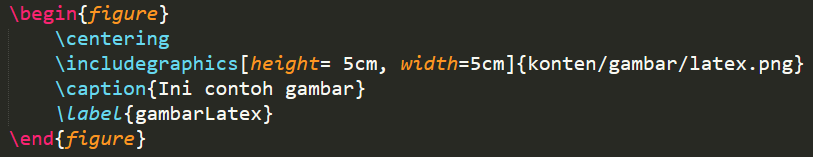
\includegraphics[height= 3cm, width=10.5cm]{konten/gambar/contohGambar.png}
	\caption{Cara memasukkan gambar di Latex}
	\label{gambarA}
\end{figure}

\begin{figure}
	\centering
	
\includegraphics[height= 5cm, width=5cm]{konten/gambar/latex.png}
	\caption{Latex itu sederhana \protect\cite{arfajsyah2018sistem}}
	\label{gambarB}
\end{figure}


Berikut hal-hal yang perlu diketahui dalam memasukkan gambar di Latex: 

\begin{enumerate}
	\item Setiap gambar harus diberikan caption dan diberikan label. 
	\item Label dapat digunakan untuk merujuk gambar tertentu dengan kode \bslash pic $\backsim$ \bslash ref $\lbrace namaLabel \rbrace$.
	\item Jika posisi gambar berubah, maka nomor gambar juga akan diubah secara 
otomatis. Begitu juga dengan seluruh kalimat yang merujuk pada gambar tersebut.
\end{enumerate}

%-----------------------------------------------------------------------------%
\section{Bagaimana Cara Membuat Tabel}
%-----------------------------------------------------------------------------%
Seperti pada gambar, tabel juga dapat diberi label dan caption. Caption pada tabel terletak pada bagian atas tabel. Contoh tabel sederhana dapat dilihat pada \tab~\ref{tabelA}. Contoh tabel dengan penggabungan baris dan penggabungan kolom dapat dilihat pada \tab~\ref{tabelB}. Contoh tabel dengan tulisan vertikal dapat dilihat pada \tab~\ref{tabelC}. Contoh tabel skenario dapat dilihat pada \tab~\ref{tabelD}. Contoh tabel \textit{landscape} dapat dilihat pada \tab~\ref{tabelE}. Contoh tabel yang ada referensinya dapat dilihat pada \tab~\ref{tabelB}.

%======================================================================%
{
\fontsize{10}{12}\selectfont
\begin{longtable}{p{3cm} p{3cm} p{3cm}}
	\caption{Contoh tabel pertama}\\
	\hline
	\textbf{Variabel A} & \textbf{Variabel B} & \textbf{Variabel C}\\
	\hline
	\endfirsthead

	\multicolumn{3}{c}{\tablename\ \thetable\ Contoh tabel pertama \space (Tabel lanjutan...)} \\
	\hline
	\textbf{Variabel A} & \textbf{Variabel B} & \textbf{Variabel C}\\
	\hline
	\endhead

	A & B & C\\
	D & E & F\\
	G & H & I\\
	J & K & L\\ \hline

\label{tabelA}
\end{longtable}
}

%=====================================================================%
{
\fontsize{10}{12}\selectfont
\begin{longtable}{p{3cm} p{4cm} p{3cm}}
	\caption{Gabung baris/kolom pada tabel \protect\cite{sari2017sistem}}\\
	\hline
	\textbf{No. Transaksi} & \textbf{Item} & \textbf{Qty}\\
	\hline
	\endfirsthead

	\multicolumn{3}{c}{\tablename\ \thetable\ Gabung baris/kolom pada tabel \protect\cite{sari2017sistem} \space (Tabel lanjutan...)} \\
	\hline
	\textbf{No. Transaksi} & \textbf{Item} & \textbf{Qty}\\
	\hline
	\endhead

	\multirow{2}{\linewidth}{1} & Mie Rebus Instan & 3\\
	 & Mie Goreng Instan & 1\\
	\multirow{3}{\linewidth}{2} & Air Mineral & 4\\
	 & Roti Coklat & 5\\
	 & Gula & 3\\
	 \hline
	\multicolumn{2}{p{7cm}}{Jumlah} & 16\\ \hline

\label{tabelB}
\end{longtable}
}


%============================================================================%
{
\fontsize{10}{12}\selectfont
\begin{longtable}{p{0.5cm} p{0.5cm} p{0.5cm} p{0.5cm} p{0.5cm} p{0.5cm} p{0.5cm} p{0.5cm} p{0.5cm} p{0.5cm}}
	\caption{Contoh tulisan vertikal pada tabel}\\
	\hline
	\textbf{No.} & \rotatebox{90}{\textbf{Item 1}} & \rotatebox{90}{\textbf{Item 2}} & \rotatebox{90}{\textbf{Item 3}} & \rotatebox{90}{\textbf{Item 4}} & \rotatebox{90}{\textbf{Item 5}} & \rotatebox{90}{\textbf{Item 6}} & \rotatebox{90}{\textbf{Item 7}} & \rotatebox{90}{\textbf{Item 8}} & \rotatebox{90}{\textbf{Item 9}}\\
	\hline
	\endfirsthead

	\multicolumn{10}{c}{\tablename\ \thetable\ Contoh tulisan vertikal pada tabel \space (Tabel lanjutan...)} \\
	\hline
	\textbf{No.} & \rotatebox{90}{\textbf{Item 1}} & \rotatebox{90}{\textbf{Item 2}} & \rotatebox{90}{\textbf{Item 3}} & \rotatebox{90}{\textbf{Item 4}} & \rotatebox{90}{\textbf{Item 5}} & \rotatebox{90}{\textbf{Item 6}} & \rotatebox{90}{\textbf{Item 7}} & \rotatebox{90}{\textbf{Item 8}} & \rotatebox{90}{\textbf{Item 9}}\\
	\hline
	\endhead

	1 & 1 & 1 & 0 & 0 & 0 & 0 & 0 & 0 & 0\\
	2 & 0 & 0 & 0 & 1 & 1 & 0 & 0 & 0 & 0\\
	3 & 0 & 0 & 0 & 0 & 0 & 0 & 0 & 1 & 1\\ \hline

\label{tabelC}
\end{longtable}
}

%=============================================================================%

{
\fontsize{10}{12}\selectfont
\begin{longtable}{p{6.5cm} p{6.5cm}}

	\caption{Contoh tabel skenario}\\
	\hline
	\multicolumn{2}{p{13cm}}{\textbf{Nama Use Case:} Disini isi nama usecase anda}\\
	\multicolumn{2}{p{13cm}}{\textbf{Deskripsi:} Disini isi deksripsi usecase anda}\\
	\multicolumn{2}{p{13cm}}{\textbf{Tujuan:} Disini isi tujuan usecase anda}\\
	\multicolumn{2}{p{13cm}}{\textbf{Aktor:} Disini isi aktor yang terlibat}\\
	\multicolumn{2}{p{13cm}}{\textbf{Kondisi Awal:} Disini isi kondisi awal}\\
	\multicolumn{2}{p{13cm}}{\textbf{Kondisi Akhir:} Disini isi kondisi akhir}\\
	\hline
	\endfirsthead

	\multicolumn{2}{c}{\tablename\ \thetable\ Contoh tabel skenario \space (Tabel lanjutan...)} \\
	\hline
	\multicolumn{2}{p{13cm}}{\textbf{Nama Use Case:} Disini isi nama usecase anda}\\
	\multicolumn{2}{p{13cm}}{\textbf{Deskripsi:} Disini isi deksripsi usecase anda}\\
	\multicolumn{2}{p{13cm}}{\textbf{Tujuan:} Disini isi tujuan usecase anda}\\
	\multicolumn{2}{p{13cm}}{\textbf{Aktor:} Disini isi aktor yang terlibat}\\
	\multicolumn{2}{p{13cm}}{\textbf{Kondisi Awal:} Disini isi kondisi awal}\\
	\multicolumn{2}{p{13cm}}{\textbf{Kondisi Akhir:} Disini isi kondisi akhir}\\
	\hline
	\endhead


	\multicolumn{2}{c}{\textbf{Skenario Normal}}\\ \hline
	\multicolumn{1}{c}{\textbf{Aksi Aktor}} & \multicolumn{1}{c}{\textbf{Aksi Sistem}}\\
	1. Aksi normal 1 & \\
	2. Aksi normal 2 &\\
	& 3. Aksi normal 3\\
	& 4. Aksi normal 4\\

	\hline
	\multicolumn{2}{c}{\textbf{Skenario Gagal}}\\ \hline
	\multicolumn{1}{c}{\textbf{Aksi Aktor}} & \multicolumn{1}{c}{\textbf{Aksi Sistem}}\\
	1. Aksi gagal 1 & \\
	2. Aksi gagal 2 &\\
	& 3. Aksi gagal 3\\
	& 4. Aksi gagal 4\\ \hline

\label{tabelD}
\end{longtable}
}

%=================================================================%
{
\fontsize{10}{12}\selectfont
\begin{landscape}
\begin{longtable}[c]{llll}
\caption{Contoh tabel landscape}
\label{tabelE}\\
\hline
\textbf{Variabel A} & \textbf{Variabel B} & \textbf{Variabel C} & \textbf{Variabel D} \\ \hline
\endfirsthead
%
\multicolumn{4}{c}%
{{\bfseries \tablename\ \thetable\ Contoh tabel landscape}} \\
\hline
\textbf{Variabel A} & \textbf{Variabel B} & \textbf{Variabel C} & \textbf{Variabel D} \\ \hline
\endhead
%
\multirow{2}{*}{A} & B & C & D \\
 & F & G & H \\
I & J & K & L \\ \hline
\end{longtable}
\end{landscape}
}


%-----------------------------------------------------------------------------------------------%
%
% Maret 2019
% Template Latex untuk Tugas Akhir Program Studi Sistem informasi ini
% dikembangkan oleh Inggih Permana (inggihjava@gmail.com)
%
% Template ini dikembangkan dari template yang dibuat oleh Andreas Febrian (Fasilkom UI 2003).
%
% Orang yang cerdas adalah orang yang paling banyak mengingat kematian.
%
%-----------------------------------------------------------------------------------------------%


%-----------------------------------------------------------------------------%
\chapter{\babTiga}
%-----------------------------------------------------------------------------%


%-----------------------------------------------------------------------------%
\section{Cara Normalisasi Data dengan Min-Max \textit{Normalization}}
%-----------------------------------------------------------------------------%
% \sqrt[3]{}
% \times = kali
% sigma = \sum

\noindent \begin{align}\label{minmax}
	\widehat{X_{i}} = \cfrac{x_{i} - x_{min}}{x_{max} - x_{min}}
\end{align}

\equ~\ref{minmax} adalah persamaan MinMax Normalization. $\widehat{X_{i}}$ adalah nilai data hasil normalisasi.

%-----------------------------------------------------------------------------%
\section{Euclidean \textit{Distance}}
\noindent \begin{align}\label{euclid}
	d = \sqrt{\sum_{i=1}^{n} (c_{i}-x_{i})^{2}}
\end{align}

\equ~\ref{euclid} adalah persamaan Euclidean \textit{Distance}.

\ifthenelse{\equal{\bidangta}{DUA}}{
  \renewcommand{\babEmpat}{ANALISIS DAN HASIL}
  \renewcommand{\babLima}{PENUTUP}  
}{}

\ifthenelse{\equal{\tipeta}{PROPOSAL TUGAS AKHIR}}{
  \renewcommand{\babEmpat}{JANGKAAN HASIL}
}{}

%-----------------------------------------------------------------------------------------------%
%
% Maret 2019
% Template Latex untuk Tugas Akhir Program Studi Sistem informasi ini
% dikembangkan oleh Inggih Permana (inggihjava@gmail.com)
%
% Template ini dikembangkan dari template yang dibuat oleh Andreas Febrian (Fasilkom UI 2003).
%
% Orang yang cerdas adalah orang yang paling banyak mengingat kematian.
%
%-----------------------------------------------------------------------------------------------%


%-----------------------------------------------------------------------------%
\chapter{\babEmpat}
%-----------------------------------------------------------------------------%
Tidak ada batasan membuat subbab pada Bab 4. Buatlah subbab sesuai kebutuhan tugas akhir anda.
%-----------------------------------------------------------------------------%
\section{Analisa}
%-----------------------------------------------------------------------------%
Buat tulisan anda disini. Buat tulisan anda disini. Buat tulisan anda disini. Buat tulisan anda disini. Buat tulisan anda disini. Buat tulisan anda disini. Buat tulisan anda disini. Buat tulisan anda disini.

\subsection{Analisa Kebutuhan Fungsional Sistem}
Buat tulisan anda disini. Buat tulisan anda disini. Buat tulisan anda disini. Buat tulisan anda disini. Buat tulisan anda disini. Buat tulisan anda disini. Buat tulisan anda disini. Buat tulisan anda disini.

\subsection{Analisa Kebutuhan Non-Fungsional Sistem}
Buat tulisan anda disini. Buat tulisan anda disini. Buat tulisan anda disini. Buat tulisan anda disini. Buat tulisan anda disini. Buat tulisan anda disini. Buat tulisan anda disini. Buat tulisan anda disini.

%-----------------------------------------------------------------------------%
\section{Perancangan}
%-----------------------------------------------------------------------------%
Buat tulisan anda disini. Buat tulisan anda disini. Buat tulisan anda disini. Buat tulisan anda disini. Buat tulisan anda disini. Buat tulisan anda disini. Buat tulisan anda disini. Buat tulisan anda disini.

\subsection{Perancangan Struktur Menu}
Buat tulisan anda disini. Buat tulisan anda disini. Buat tulisan anda disini. Buat tulisan anda disini. Buat tulisan anda disini. Buat tulisan anda disini. Buat tulisan anda disini. Buat tulisan anda disini.

\subsection{Perancangan Basis Data}
Buat tulisan anda disini. Buat tulisan anda disini. Buat tulisan anda disini. Buat tulisan anda disini. Buat tulisan anda disini. Buat tulisan anda disini. Buat tulisan anda disini. Buat tulisan anda disini.

\subsection{Perancangan Antar-Muka}
Buat tulisan anda disini. Buat tulisan anda disini. Buat tulisan anda disini. Buat tulisan anda disini. Buat tulisan anda disini.

\ifthenelse{\equal{\tipeta}{TUGAS AKHIR}}{
  %-----------------------------------------------------------------------------------------------%
%
% Maret 2019
% Template Latex untuk Tugas Akhir Program Studi Sistem informasi ini
% dikembangkan oleh Inggih Permana (inggihjava@gmail.com)
%
% Template ini dikembangkan dari template yang dibuat oleh Andreas Febrian (Fasilkom UI 2003).
%
% Orang yang cerdas adalah orang yang paling banyak mengingat kematian.
%
%-----------------------------------------------------------------------------------------------%

%-----------------------------------------------------------------------------%
\chapter{\babLima}
%-----------------------------------------------------------------------------%
Tidak ada batasan membuat subbab pada Bab 5. Buatlah subbab sesuai kebutuhan tugas akhir anda.

%-----------------------------------------------------------------------------%
\section{Hasil Implementasi}
%-----------------------------------------------------------------------------%
Buat tulisan anda disini. Buat tulisan anda disini. Buat tulisan anda disini. Buat tulisan anda disini. Buat tulisan anda disini. Buat tulisan anda disini. Buat tulisan anda disini. Buat tulisan anda disini.

%-----------------------------------------------------------------------------%
\section{Hasil Penguji}
%-----------------------------------------------------------------------------%
Buat tulisan anda disini. Buat tulisan anda disini. Buat tulisan anda disini. Buat tulisan anda disini. Buat tulisan anda disini. Buat tulisan anda disini. Buat tulisan anda disini. Buat tulisan anda disini.
  \ifthenelse{\equal{\bidangta}{SATU}}{
    %-----------------------------------------------------------------------------------------------%
%
% Maret 2019
% Template Latex untuk Tugas Akhir Program Studi Sistem informasi ini
% dikembangkan oleh Inggih Permana (inggihjava@gmail.com)
%
% Template ini dikembangkan dari template yang dibuat oleh Andreas Febrian (Fasilkom UI 2003).
%
% Orang yang cerdas adalah orang yang paling banyak mengingat kematian.
%
%-----------------------------------------------------------------------------------------------%


%-----------------------------------------------------------------------------%
\chapter{\babEnam}
%-----------------------------------------------------------------------------%
\section{Kesimpulan}
Kesimpulan dari penelitian ini adalah:
\begin{enumerate}
	\item Hidup di dunia pasti mati.
	\item Kehidupan di akhirat adalah kehidupan abadi.
	\item Semoga dosa kita diampuni oleh Allah SWT.
\end{enumerate}
\section{Saran}
Saran dari penelitian ini adalah:
\begin{enumerate}
	\item Jagalah sholatmu.
	\item Hindari berbuat dosa.
	\item Perbanyak perbuat pahala.
	\item Semoga dosa kita diampuni oleh Allah SWT.
\end{enumerate}


  }{}
}{}

\bibliographystyle{apacite} 
\renewcommand{\bibname}{DAFTAR PUSTAKA}
\bibliography{konfigurasi/daftarpustaka}
\clearpage

\begin{appendix}
\begin{appendices}	
\renewcommand{\appendixname}{LAMPIRAN}
\renewcommand{\chaptername}{LAMPIRAN}
  \setcounter{page}{1}
%-----------------------------------------------------------------------------------------------%
%
% Maret 2019
% Template Latex untuk Tugas Akhir Program Studi Sistem informasi ini
% dikembangkan oleh Inggih Permana (inggihjava@gmail.com)
%
% Template ini dikembangkan dari template yang dibuat oleh Andreas Febrian (Fasilkom UI 2003).
%
% Orang yang cerdas adalah orang yang paling banyak mengingat kematian.
%
%-----------------------------------------------------------------------------------------------%

%-----------------------------------------------------------------------------%
%\prefikLampiran{A}
\renewcommand{\thepage}{A - \arabic{page}}
\chapter{HASIL WAWANCARA}
%-----------------------------------------------------------------------------%


\setcounter{page}{1}
%-----------------------------------------------------------------------------------------------%
%
% Maret 2019
% Template Latex untuk Tugas Akhir Program Studi Sistem informasi ini
% dikembangkan oleh Inggih Permana (inggihjava@gmail.com)
%
% Template ini dikembangkan dari template yang dibuat oleh Andreas Febrian (Fasilkom UI 2003).
%
% Orang yang cerdas adalah orang yang paling banyak mengingat kematian.
%
%-----------------------------------------------------------------------------------------------%

%-----------------------------------------------------------------------------%
%\prefikLampiran{A}

\renewcommand{\thepage}{B - \arabic{page}}
\chapter{HASIL OBSERVASI}
%-----------------------------------------------------------------------------%

\setcounter{page}{1}
%-----------------------------------------------------------------------------------------------%
%
% Maret 2019
% Template Latex untuk Tugas Akhir Program Studi Sistem informasi ini
% dikembangkan oleh Inggih Permana (inggihjava@gmail.com)
%
% Template ini dikembangkan dari template yang dibuat oleh Andreas Febrian (Fasilkom UI 2003).
%
% Orang yang cerdas adalah orang yang paling banyak mengingat kematian.
%
%-----------------------------------------------------------------------------------------------%

%-----------------------------------------------------------------------------%
%\prefikLampiran{A}

\renewcommand{\thepage}{C - \arabic{page}}
\chapter{DATA MORFOMETRIK SAPI}
%-----------------------------------------------------------------------------%

\setcounter{page}{1}
%-----------------------------------------------------------------------------------------------%
%
% Maret 2019
% Template Latex untuk Tugas Akhir Program Studi Sistem informasi ini
% dikembangkan oleh Inggih Permana (inggihjava@gmail.com)
%
% Template ini dikembangkan dari template yang dibuat oleh Andreas Febrian (Fasilkom UI 2003).
%
% Orang yang cerdas adalah orang yang paling banyak mengingat kematian.
%
%-----------------------------------------------------------------------------------------------%

%-----------------------------------------------------------------------------%
%\prefikLampiran{A}

\renewcommand{\thepage}{D - \arabic{page}}
\chapter{HASIL UJI UAT}
%-----------------------------------------------------------------------------%

XYZasdasd
\end{appendices}
\end{appendix}

\ifthenelse{\equal{\tipeta}{TUGAS AKHIR}}{
    %-----------------------------------------------------------------------------------------------%
%
% Maret 2019
% Template Latex untuk Tugas Akhir Program Studi Sistem informasi ini
% dikembangkan oleh Inggih Permana (inggihjava@gmail.com)
%
% Template ini dikembangkan dari template yang dibuat oleh Andreas Febrian (Fasilkom UI 2003).
%
% Orang yang cerdas adalah orang yang paling banyak mengingat kematian.
%
%-----------------------------------------------------------------------------------------------%

\chapter*{DAFTAR RIWAYAT HIDUP}
\pagestyle{empty}

\noindent
\begin{wrapfigure}{l}{3cm}

\includegraphics[width=3cm, height=4cm]{konten/gambar/fotoprofil.jpg}
\end{wrapfigure}
Tulis daftar riwayat hidup anda disini. Tulis daftar riwayat hidup anda disini. Tulis daftar riwayat hidup anda disini. Tulis daftar riwayat hidup anda disini. Tulis daftar riwayat hidup anda disini. Tulis daftar riwayat hidup anda disini. Tulis daftar riwayat hidup anda disini.
Tulis daftar riwayat hidup anda disini. Tulis daftar riwayat hidup anda disini. Tulis daftar riwayat hidup anda disini. Tulis daftar riwayat hidup anda disini. Tulis daftar riwayat hidup anda disini. Tulis daftar riwayat hidup anda disini. Tulis daftar riwayat hidup anda disini.
Tulis daftar riwayat hidup anda disini. Tulis daftar riwayat hidup anda disini. Tulis daftar riwayat hidup anda disini. Tulis daftar riwayat hidup anda disini. Tulis daftar riwayat hidup anda disini. Tulis daftar riwayat hidup anda disini. Tulis daftar riwayat hidup anda disini.
}{}    

\end{document}